\documentclass{ieeetj}
\usepackage{cite}
\usepackage{amsmath,amssymb,amsfonts}
\usepackage{algorithmic}
\usepackage{graphicx,color}
\usepackage{textcomp}
\usepackage{xcolor}
\usepackage{hyperref}
\hypersetup{hidelinks=true}
\usepackage{algorithm,algorithmic}
\def\BibTeX{{\rm B\kern-.05em{\sc i\kern-.025em b}\kern-.08em
    T\kern-.1667em\lower.7ex\hbox{E}\kern-.125emX}}
\AtBeginDocument{\definecolor{tmlcncolor}{cmyk}{0.93,0.59,0.15,0.02}\definecolor{NavyBlue}{RGB}{0,86,125}}




\def\OJlogo{\vspace{-4pt}$<$Society logo(s) and publication title will appear here.$>$}
\def\seclogo{\vspace{10pt}$<$Society logo(s) and publication title will appear here.$>$}

\def\authorrefmark#1{\ensuremath{^{\textbf{#1}}}}

\begin{document}
\receiveddate{XX Month, XXXX}
\reviseddate{XX Month, XXXX}
\accepteddate{XX Month, XXXX}
\publisheddate{XX Month, XXXX}
\currentdate{XX Month, XXXX}
\doiinfo{XXXX.2022.1234567}

\markboth{}{Author {et al.}}

\title{A Review of Traditional Financial Models and Mandelbrotian Alternatives}

\author{Gergely Madarász, Róbert Cserpák, Márton Páll}


\begin{abstract}
Traditional financial models rely on the normal distribution assumption to describe market behavior, yet this foundation is fundamentally flawed.
Drawing from the works of Nassim Taleb\cite{taleb2025} and Benoit Mandelbrot\cite{mandelbrot2004}, this paper examines why conventional models like Black-Scholes and the Sharpe ratio fail to capture market realities that consistently exhibit fat tails, asymmetry, and volatility clustering.

This review explores the empirical evidence suggesting that financial markets display power-law behaviors and long-range dependencies that contradict the independence and normality assumptions underlying traditional models.
The implications extend beyond theoretical concerns to practical issues in risk assessment, where underestimating tail probabilities can lead to substantial losses.

As an alternative, we review Mandelbrot's Fractal Market Hypothesis, incorporating scaling laws and multifractal properties to model financial markets' complex nature. This approach acknowledges the hierarchical structure of market volatility and the presence of multiple time scales in price dynamics.
Combined with Taleb's work on fat-tailed distributions, fractal-based approaches represent a paradigm shift toward more accurate financial modeling with significant implications for risk management and derivative pricing.
\end{abstract}

\begin{IEEEkeywords}
Fractal Market Hypothesis, fat-tailed distributions, Black-Scholes limitations, financial modeling, power laws, risk management, Sharpe Ratio
\end{IEEEkeywords}

%\IEEEspecialpapernotice{(Invited Paper)}

\maketitle

\section{INTRODUCTION}
\subsection{The Dominance of the Gaussian Paradigm}
Traditional financial models rely on the \textbf{normal distribution assumption} to describe market behavior. The earliest and foundational random-walk model for security markets was constructed by Louis Bachelier (1900)\cite{mandelbrot1963variation}, who posited that successive price differences are \textbf{independent, Gaussian or normally distributed}\cite{mandelbrot1963variation}. This stochastic process came to be called "Brownian motion"\cite{mandelbrot1963variation}. This Gaussian assumption, with its implication of finite moments, underpins conventional approaches. The development of option pricing was later influenced by Jack L. Treynor, leading to the Black-Scholes\cite{blackscholes1973} (B-S) option pricing model. An option is defined as a security granting the right to buy or sell an asset subject to certain conditions within a specified period. The B-S model relies on the premise that the return on the underlying security has a \textbf{normal distribution with a constant variance rate ($\sigma^2$
 )} through time. The variance rate is mathematically defined as the limit of the return's variance over an interval, divided by the length of the interval, as the interval size approaches zero.

\subsection{Traditional Risk Metrics and Limitations}
The reliance on the Gaussian assumption extends directly to measures of risk and portfolio management, such as the Sharpe ratio, Value at Risk (VaR), and Kurtosis \cite{taleb2025}. The most basic prerequisite for standard statistical analysis of market data is the\textbf{ stationarity hypothesis}, which assumes that core statistical properties remain stable over time. However, the foundational assumption of the Gaussian model is fundamentally flawed. Empirical studies suggest that financial price changes are typically \textbf{too "peaked"} to be samples drawn from Gaussian populations. Furthermore, the B-S model's key assumption of a constant variance rate ($\sigma^2$) is contradicted by empirical evidence, which suggests that the variance rate changes over time. The failure to understand the true \textbf{consequences of fat tails} renders traditional statistics derived from the Gaussian framework (like variance and the Sharpe ratio) ineffective or misleading. In fact, in the reality of \textbf{Extremistan} (thick tails), \textbf{rare events play a disproportionately large role} in determining the distribution's properties, fundamentally challenging the stable nature assumed in \textbf{Mediocristan} (thin tails).

\subsection{Overview}
Drawing from the works of Nassim Taleb and Benoit Mandelbrot, this paper argues that the instability and unreliability of these traditional models necessitate a paradigm shift. The inadequacy of conventional models like Black-Scholes and the Sharpe ratio stems from their inability to capture market realities that consistently exhibit \textbf{fat tails, asymmetry, and volatility clustering}. This paper advocates moving beyond models reliant on assumptions of independence and finite moments towards frameworks, such as stable Paretian laws introduced by Mandelbrot, that incorporate the empirical evidence of fat tails and scaling laws \cite{mandelbrot1963variation}. The central goal is to address the\textbf{ statistical consequences of fat tails}, by reviewing Mandelbrot’s Fractal Market Hypothesis and related approaches, which offer a more accurate methodology for financial modeling, risk management, and derivative pricing.

\section{Critique of Traditional Valuation Models}

\subsection{The Black-Scholes (B-S) Option Pricing Model and its Idealizations}
The Black-Scholes (B-S) option pricing model serves as a cornerstone of conventional financial theory. An option is formally defined as a security granting the right to buy or sell an asset subject to certain conditions within a specified period of time. Specifically, a European option can be exercised only on a specified future date. The B-S model relies on several core idealizations regarding the underlying asset’s price movement and the market environment.

Firstly, the model assumes that the return on the underlying security has a \textbf{normal distribution} \cite{macbethmerville1979}. Secondly, it posits that this distribution is characterized by a \textbf{constant variance rate} ($\sigma^2$) through time. The variance rate itself is mathematically defined as the limit, as the measurement interval approaches zero, of the return’s variance over that interval divided by the length of the interval.

 In addition to these distributional assumptions, the B-S framework assumes an idealized trading environment: there are \textbf{no transaction costs} in buying or selling the option or the underlying security, \textbf{no taxes}, and \textbf{no restrictions on short sales}.

 The method employed by B-S to determine the option’s value hinges on the concept of continuous dynamic hedging. This procedure theoretically allows for the creation of a continuously adjusted, riskless hedged position. Crucially, because the risk of this hedged position is entirely diversifiable, its \textbf{expected return must be equivalent to the short-term interest rate}. This technique fundamentally removes the need for a risk premium in the valuation process.

 However, the empirical application and the theoretical rigor of the B-S model quickly break down when tested against real-world markets. The valuation relies on the assumption that continuous dynamic hedging is possible, a procedure that is mathematically impossible in a fat-tailed environment. Furthermore, empirical examination of market data reveals that observed rates of return suggest a changing variance rate, contradicting the model's assumption of constant $\sigma^2$. Tests have indicated that option prices bought and sold in the market deviate from the prices predicted by the B-S formula in\textbf{ certain systematic ways}. For instance, option buyers consistently pay prices that are higher than those predicted by the B-S formula.


\subsection{The Instability of Variance and the Sharpe Ratio}
The critique of traditional modeling extends beyond the technical assumptions of option pricing to the core statistical foundations of risk measurement, primarily the reliance on the \textbf{normal distribution} assumption. Financial markets consistently exhibit \textbf{fat tails} and volatility clustering, realities that the Gaussian framework fails to capture.

Benoit Mandelbrot’s early observations highlighted the insufficiency of the normal distribution, noting that the empirical distributions of price changes are usually\textbf{ too "peaked"} compared to Gaussian populations. Furthermore, the tails of these distributions are so extraordinarily long that the resulting \textbf{sample second moments} (variance) vary in an erratic fashion and appear \textbf{statistically unstable}. For example, historical data on cotton prices demonstrated that the sample variance did not converge to a stable limit as the sample size increased, leading to the hypothesis that the \textbf{theoretical variance may be infinite}. In situations characterized by thick tails, financial data exhibits significantly positive kurtosis, suggesting that the fourth moment is statistically unstable or nonexistent. The use of metrics like the variance or standard deviation relies on the assumption of \textbf{finite and stable moments}, which heavy-tailed data violate.

This instability directly undermines the efficacy of widely used performance metrics, such as the Sharpe ratio. The Sharpe ratio calculates expected return divided by the \textbf{standard deviation (STD)}, using STD as the predominant measure of risk. This reliance on standard deviation is often criticized because it assumes a \textbf{symmetrical return distribution} and penalizes upside deviations (positive volatility) just as much as downside deviations (negative volatility).

When distributions are fat-tailed or non-normal (especially negatively skewed), the Sharpe ratio becomes \textbf{ill-suited} and potentially \textbf{uninformative}. In the search for metrics that address this fundamental flaw, measures focused specifically on downside risk have emerged. Downside deviation, the risk measure employed in the Sortino ratio, quantifies the deviation of returns that fall \textbf{below the mean} (or a specified target rate), making it appropriate for analyzing non-normal and asymmetric distributions where the primary concern is managing negative outcomes. The persistence of fat tails implies that risk management protocols based solely on traditional variance measures fail to assess \textbf{tail probabilities}, leading to the risk of substantial losses.


\section{Empirical Evidence of Non-Normality and Long-Range Dependence }
\subsection{The Statistical Characteristics of Fat Tails (Heavy Tails)}

The fundamental reliance of traditional financial models on the normal distribution assumption is contradicted by persistent empirical observations showing that market returns display \textbf{heavy-tailed} characteristics. Financial time series analysis necessarily begins by defining the core variable of interest, the \textbf{log return}. Given $S(t)$ as the price of a financial asset and $X(t)=lnS(t)$ as its logarithm, the log return $r(t,\Delta{t})$ over a time scale $\Delta{t}$ is formally defined as:

$$r(t,\Delta{t})=X(t+\Delta{t})-X(t)$$

Early research, particularly by Benoit Mandelbrot in the 1960s, pointed out the insufficiency of the normal distribution for modeling the marginal distribution of asset returns due to their heavy-tailed character. The unconditional distribution of returns is consistently found to be \textbf{non-Gaussian, sharp-peaked, and heavy-tailed}.

\begin{figure}
    \centering
    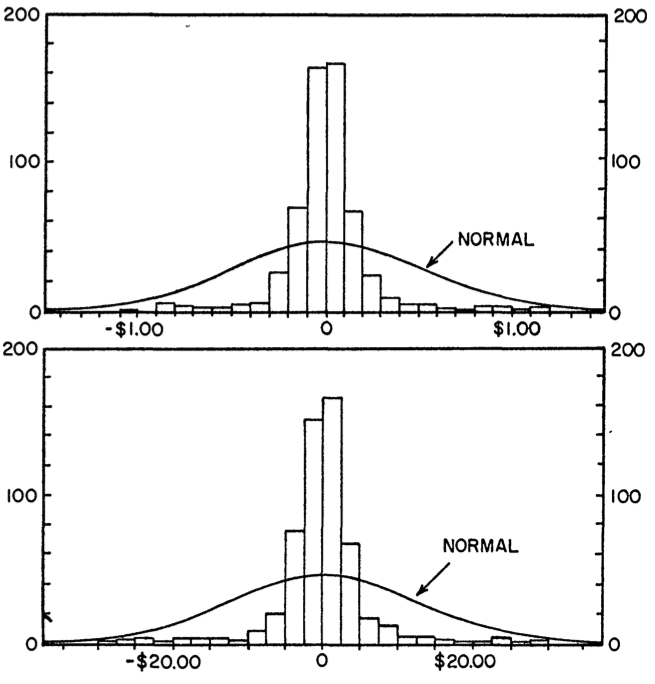
\includegraphics[width=1\linewidth]{heavy_tailed.png}
    \caption{Two histograms illustrating departure from normality of the fifth and tenth difference of monthly wool prices, 1890-1937. In each case, the continuous bell-shaped curve represents the Gaussian "interpolate" based upon the sample variance. Source: Gerhard Tintner, The Variate-Difference dence and Method (Bloomington, Ind., 1940)}
    \label{fig:placeholder}
\end{figure}



\subsubsection{Quantification of Deviation: Kurtosis Data}

To quantitatively reject the Gaussian paradigm, researchers rely on the \textbf{kurtosis} ($\kappa$), a measure of the distribution’s tail fatness and peak sharpness relative to the normal distribution. When measured as \textit{excess kurtosis} (raw kurtosis minus 3), the value for a Gaussian distribution is $\kappa=0$.

Empirical studies consistently show that the kurtosis of asset prices is significantly positive, far exceeding the Gaussian benchmark. This effect is especially pronounced for fine (intraday) time scales. Typical observed values for the excess kurtosis in financial data are dramatic, providing strong evidence of fat tails:

\begin{itemize}
    \item For 5-minute price increments, observed kurtosis values range significantly.
    \item The \textbf{S\&P 500 index futures} exhibited a kurtosis ($\kappa$) of approximately 16.
    \item \textbf{US\$/Swiss Franc exchange rate futures} displayed a kurtosis of approximately 60.
    \item \textbf{US\$/DM exchange rate futures} registered values as high as 74.
\end{itemize}

This quantitative evidence firmly places financial returns outside the thin-tailed domain assumed by traditional models, confirming that large deviations occur far more frequently than predicted by a normal distribution.

\subsubsection{Implication for Moment Instability}

This departure from Gaussian thin tails leads directly to severe consequences for standard statistical measures. The instability of higher moments (moments beyond the mean, such as variance, which is the second moment, and kurtosis, which relates to the fourth moment) highlights that their measurement in thick-tailed domains is often unreliable or meaningless. The reliance on variance (or standard deviation) assumes moments of the distribution are finite and stable.
The instability of higher moments is starkly illustrated by examining the dominant influence of single extreme events:

\begin{itemize}
    \item A single observation may contribute overwhelmingly to the total kurtosis, implying the fourth moment is statistically unstable or may not exist.
    \item For the\textbf{ S\&P 500 index}, the concentration of kurtosis in the single market movement of the \textbf{1987 crash determined 80\% of the total kurtosis over a 50-year period}.
\end{itemize}


This instability reinforces the critique that traditional risk metrics cannot function reliably. If the fourth moment is statistically unstable or non-existent, the measurement itself is compromised. This outcome demonstrates the extreme fragility of conventional statistics under fat tails, where the presence of a few rare, large events dictates the estimated statistical properties, rendering measures like the variance based on the assumption of stability, fundamentally invalid for robust financial analysis.

\subsection{The Preasymptotics Problem and Data Sufficiency}

The foundational structure of traditional mathematical statistics is built upon the assumption of \textbf{asymptotic behavior}. Convergence theorems, notably the \textbf{Central Limit Theorem (CLT)} and the \textbf{Law of Large Numbers (LLN)}, guarantee that sample statistics approach their theoretical population values when the number of observations ($n$) approaches infinity ($n\to \inf$). The LLN, for instance, tells us that as the number of independent, identically distributed random variables increases, their sample average converges to the expected value ($\mu$).

However, the applicability of these asymptotic guarantees is severely compromised in the real world, a domain formalized by the critical concept of \textbf{Preasymptotics}. The preasymptotic domain describes the behavior of a sum or sequence when the number of summands ($n$) is large but definitively finite. This leads to the fundamental insight that \textbf{"Life happens in the preasymptotics"}.

Under thin-tailed distributions, convergence is rapid, meaning the asymptotic approximation holds well even for moderate sample sizes. Conversely, when modeling real-world financial data characterized by \textbf{fat tails}, the expected convergence is "excruciatingly slow". This phenomenon is referred to as the \textbf{"Law of Medium Numbers"}. Even if the LLN is theoretically satisfied (i.e., the mean and variance exist), it works \textbf{too slowly in the real world} to be useful for real-world time scales.

The consequences of this slow convergence are terminal for conventional inference: the instability means that the mean of the distribution rarely corresponds to the observed sample mean due to the persistent, disproportionate influence of rare events. This instability effectively \textbf{cancels most statistical estimators}.

The magnitude of this problem highlights the insufficiency of data in practical scenarios. The amount of data required for reliable statistical inference under fat tails is orders of magnitude greater than that needed for a Gaussian distribution. For example, the Pareto distribution corresponding to the famous "80/20" rule (which maps to a tail exponent $\alpha \approx 1.14$) requires $>10^9$ \textbf{more observations} than the Gaussian to reach the same level of stabilization around the mean. While the Gaussian requires only approximately 30 observations to stabilize the mean, the "Pareto 80/20" needs about $10^{11}$ observations to achieve an equivalent drop in error around the mean. This data insufficiency renders standard sample statistics meaningless for real-world time scales.

\subsection{Dependence Properties: Volatility Clustering and Intermittency}

Beyond the challenge posed by heavy-tailed marginal distributions, the foundation of traditional financial models is further undermined by complex dependence structures in financial time series, which contradict the fundamental assumption of \textbf{statistical independence} necessary for simple stochastic models.

\subsubsection{Breakdown of the Independence Assumption}

In liquid financial markets, studies consistently show that linear autocorrelations of asset returns typically \textbf{decay rapidly to zero}. This observation supports the original concept of the "efficient market hypothesis" or the \textbf{"random walk" theory}, suggesting that past movements cannot be used to predict the direction of future price changes. Benoit Mandelbrot summarized this fact by stating that \textbf{arbitrage tends to "whiten the spectrum of price changes"}.

However, the absence of serial correlation in returns does \textbf{not} imply statistical independence of the price increments. Independence would require that any nonlinear function of returns must also exhibit no autocorrelation. This property is consistently violated in financial data. Empirical studies demonstrate a strong interdependence between distant samples, suggesting that the theoretical \textbf{"span of interdependence"} between increments can be infinite, contrasting sharply with the conventional assumption of asymptotic independence. Consequently, log prices are \textbf{not} random walks.

\subsubsection{Volatility Clustering: The Signature of Nonlinear Dependence}

The primary observable signature of this underlying nonlinear dependence is \textbf{volatility clustering.} This phenomenon means that \textbf{large price variations are more likely to be followed by large variations} (and small variations by small ones). Volatility clustering is a direct empirical contradiction to the fundamental assumption in traditional models, such as the Black-Scholes-Merton (BSM) formula, which requires a \textbf{constant variance rate} ($\sigma^2$) through time.
 
This nonlinear dependence is rigorously quantified by examining the \textbf{autocorrelation of simple nonlinear functions of returns}, such as absolute returns or squared returns\cite{cont2001}. These nonlinear functions exhibit\textbf{ significant positive autocorrelation or persistence} over time. The autocorrelation function of powers of returns often displays a \textbf{slow decay}—well reproduced by a power law—suggesting \textbf{long-range dependence in volatility} that spans several days, sometimes weeks. Specifically, studies show that the autocorrelation function of absolute or squared returns follows a power law decay $C(\tau)\sim A/\tau^{\beta}$
 , with the exponent $\beta$ typically observed to be in the range of [0.2, 0.4]. The existence of such dependencies highlights that variance is inherently non-stationary and confirms the insufficiency of traditional linear random walk models.

 \begin{figure}
     \centering
     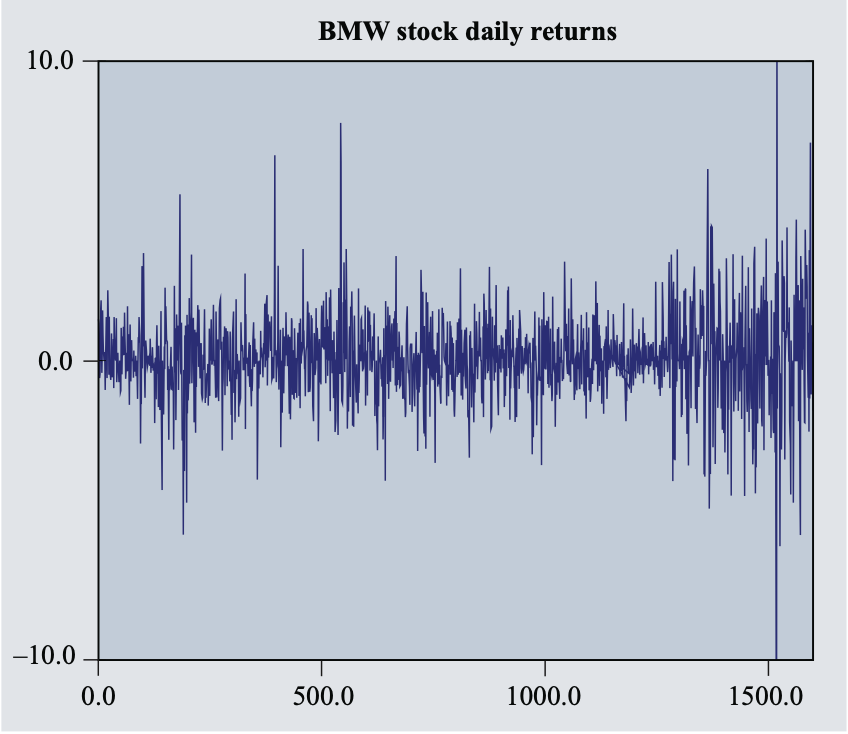
\includegraphics[width=1\linewidth]{daily_returns_of_bmw.png}
     \caption{Daily returns of BMW shares on the Frankfurt Stock Exchange, 1992-1998, Source: \cite{cont2001}}
     \label{fig:placeholder}
 \end{figure}

\subsection{Scaling Laws and Fractional Brownian Motion (fBm)}

The evidence of persistent dependence and non-normality led to the exploration of scaling properties and generalized stochastic processes, notably the introduction of \textbf{Fractional Brownian Motions (fBm's)} by Mandelbrot.

Fractional Brownian Motions were proposed as a family of Gaussian random functions designed to model time series where the \textbf{"span of interdependence"} between increments is infinite, moving beyond processes that rely on asymptotic independence. The fBm is defined using a parameter $H$ (where $0<H<1$), known as the Hurst exponent or scaling parameter. Traditional Brownian motion, used in the theoretical foundations of modern finance, is merely a specific case of fBm where $H=1/2$.

The key property of fBm is \textbf{self-similarity} (s-s), which is a form of invariance with respect to changes in the time scale. For a process with s-s increments, the distribution of returns remains the same across different measurement periods (such as days or weeks), varying only by a scale factor related to the exponent $H$. Specifically, self-similar increments satisfy

$$\{X(t_{0}+\tau,\omega)\}-X(t_{0},\omega)\sim \{h^{H}[X(t_{0}+h\tau,\omega)-X(t_{0},\omega)]\}$$ for any scaling factor $h>0$.

When the Hurst exponent falls in the range $1/2<H<1$, the process exhibits long-range dependence or "infinite memory". This property is crucial as empirical findings, such as those by Hurst regarding accumulated geophysical and hydrological series, frequently showed that the statistical range of fluctuations was proportional to $T^H$, with $H$ values often falling within this range (i.e., $1/2<H<1$).
 
If the underlying financial process were instead modeled using a \textbf{non-Gaussian self-similar process} (like Fractional Lévy-stable random functions), its increments would inherently require \textbf{infinite variance} to account for the thickness of the tails and the infinite span of interdependence. This necessity bridges the concepts of scaling behavior and the observed statistical characteristics of asset returns.


\begin{figure}
    \centering
    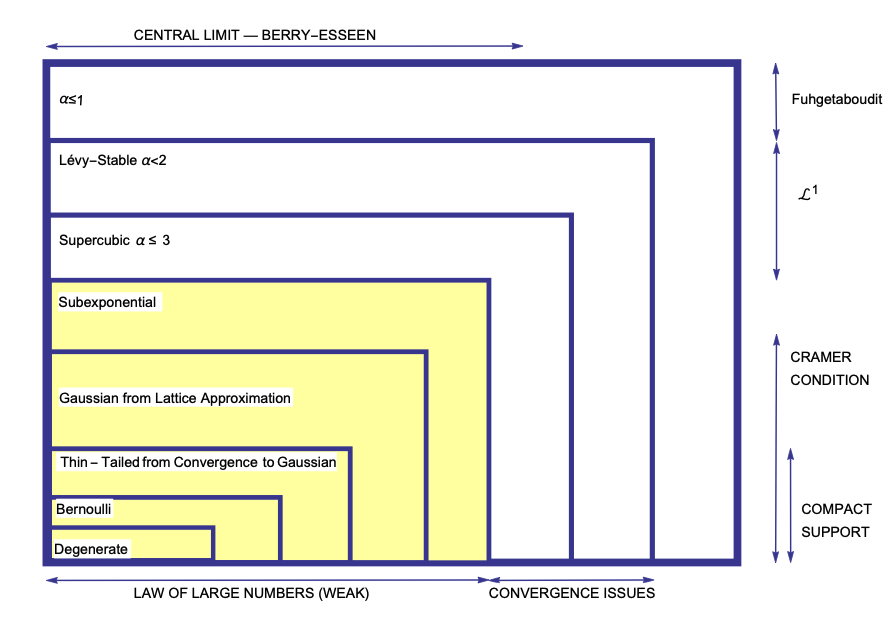
\includegraphics[width=1\linewidth]{tablue_of_thick_tails.png}
    \caption{Enter Caption}
    \label{fig:placeholder}
\end{figure}

\section{The Fractal Market Hypothesis and Alternatives}

\subsection{Mandelbrot’s Stable Paretian Approach}

The persistent failure of traditional financial models to capture fundamental market phenomena such as fat tails and volatility clustering necessitates a paradigm shift toward frameworks that acknowledge asset price complexity. Benoit Mandelbrot pioneered this shift by arguing that the empirical facts surrounding moments and market variations warrant a radically new approach to the problem of price variation, replacing the Gaussian distributions with \textbf{Stable Paretian laws}.

The Stable Paretian laws, first described by Paul Lévy, generalize the Gaussian distribution and define a family of probability distributions that are \textbf{stable under summation}. This class of laws is required to model erratic behavior in time series where sample moments fluctuate persistently, thereby necessitating the conjecture that population moments may be infinite. If the distribution of logarithmic price relatives falls into this class, price increments over different time scales (days, weeks, months) exhibit the same distribution, differing only in their scale parameters.

Crucially, the fractal and stable Paretian approaches incorporate scaling laws and inherently thick tails. If the Stable Paretian exponent $\alpha$ falls within the range of $1 < \alpha \le2$, the distribution possesses a finite mean but an infinite or undefined variance. This directly challenges the reliance on variance-based risk metrics that assume finite second moments.

The concept of scaling further formalizes market irregularity. Mandelbrot introduced the property of \textbf{self-similarity} (s-s), meaning the span of interdependence can be infinite, often described using \textbf{Fractional Lévy-stable random functions}. Under this model, the price changes follow a generalized power law, where the expected scale factor of the price change over $T$ days is proportional to $T^{1 / \alpha}\sigma(1)$, generalizing the classical $T^{1/2}$
  law of the Gaussian model. Furthermore, the fractal approach requires modeling the \textbf{price path irregularity}, as risk is fundamentally related to the local smoothness or roughness of the trajectory.

\subsection{Taleb’s Framework: Consequences of Extremistan}

Nassim Taleb's work draws on these fat-tailed foundations to detail the \textbf{statistical and epistemological consequences} of operating in the world of thick tails, termed \textbf{Extremistan}, which contrasts sharply with the thin-tailed domain of Mediocristan. The core argument is that the problem in financial modeling is not merely awareness of fat tails, but the profound \textbf{lack of understanding of their consequences}.

In the domain of Extremistan, the tails (rare events) play a \textbf{disproportionately large role} in determining the statistical properties of the series. This characteristic has immediate practical consequences:

\begin{enumerate}
    \item \textbf{Failure of the Law of Large Numbers (LLN)}: Due to thick tails, the LLN works too slowly in the real world. The mean of the distribution rarely corresponds to the observed sample mean because rare events persistently influence the average, even in large samples. This fundamental instability renders most conventional statistical estimators, including variance and correlation, uninformative out-of-sample.

    \item \textbf{Payoff Swamps Probability}: In Extremistan, high-consequence rare events dominate the cumulative outcome, dictating that decision-making should shift focus from \textit{frequency} (probability) to the expected \textit{impact} (payoff). For processes driven by thick tails (such as pandemics or systemic financial risks), risk management must focus on \textbf{reducing the effect} should a large event take place, rather than solely reducing the event's probability.
\end{enumerate}


This framework implies an\textbf{ epistemological asymmetry}: models relying on thin tails (Mediocristan) can be readily \textbf{ruled out} by observing a single large deviation (e.g., a "ten-sigma" event), while the reverse confirmation—proving a distribution is genuinely thin-tailed—is nearly impossible in finite time. This focus on robustness, utilizing statistical findings on fat tails, is necessary for developing risk management and derivative pricing protocols that avoid substantial losses associated with underestimating tail probabilities.

\section{Practical Implications for Risk Management and Pricing}

\subsection{Risk Assessment Beyond Variance}

Traditional risk assessment is fundamentally compromised by the characteristics of heavy-tailed distributions observed in financial markets. The reliance on the concept of \textbf{finite and stable moments }inherent in Gaussian models is violated by asset return data.

The instability of higher moments, particularly the fourth moment (kurtosis), severely compromises standard statistical risk estimation. In thick-tailed domains, even when a theoretical moment exists, a single observation may contribute so overwhelmingly to the total kurtosis that the fourth moment is rendered statistically unstable or nonexistent. This pervasive instability means that the statistical properties of complex metrics, such as the autocorrelation function of squared returns used to measure volatility clustering, are compromised due to the lack of a stable fourth moment.

This instability directly impacts modern regulatory measures:
\begin{itemize}
    \item \textbf{Value at Risk (VaR)}: The calculation of Value-at-Risk (VaR) requires knowledge of the \textbf{tail behavior} of the distribution of returns, as VaR is defined as a high quantile of the loss distribution over a given time horizon. Since VaR is required to determine regulatory capital requirements, mis-specification of the tail behavior carries significant consequences.
    \item \textbf{Underestimation of Tail Risk}: When the normal distribution assumption is used, risk management protocols systematically underestimate \textbf{tail probabilities}, a practice that leads to the risk of substantial losses.
\end{itemize}

\subsection{The Role of Extreme Value Theory (EVT)}

Given the demonstrable failure of traditional statistical metrics to cope with the heavy tails and moment instability characteristic of financial returns, a necessary paradigm shift involves adopting rigorous statistical tools specifically designed for the domain of extreme events. \textbf{Extreme Value Theory (EVT)} provides the mathematical framework required to deal with market extremes and the crucial task of \textbf{extrapolating past the observed sample maximum}.

The importance of EVT stems from the reality that large market movements are highly consequential and \textbf{cannot be discarded as simple outliers}. These violent market movements command the attention of participants because their magnitude often constitutes an important fraction of the aggregate return over long periods. Thus, EVT is directly relevant for risk management purposes, particularly for the accurate calculation of \textbf{Value-at-Risk (VaR)}, which is required for regulatory capital determination.

EVT approaches the problem of modeling tails by analyzing either the distribution of maximal returns over defined periods (block maxima method) or, more powerfully, the distribution of extreme values that \textbf{exceed a high threshold} (Peaks-Over-Threshold, or POT method).

The central significance of the POT method lies in the \textbf{Picklands-Balkema-de Haan Theorem}. This theorem provides an asymptotic justification for modeling these exceedances over a threshold ($u$) using a specific functional form: the \textbf{Generalized Pareto Distribution (GPD)}.

When applying EVT to financial data (such as daily returns of stocks or indices), the analysis typically yields an \textbf{extreme value index} ($\xi$) that is positive ($\xi>0$). A positive $\xi$ indicates that the distribution belongs to the \textbf{Fréchet class} of extreme values, confirming the heavy-tailed nature of the returns. For distributions with a power-law tail with exponent $\alpha$, the distribution falls in the Fréchet class, and $\xi$ is directly related to the tail index, where $\xi=1/\alpha$.

By utilizing EVT, financial modeling gains a scientifically rigorous methodology to handle the highly variable and disruptive tail risks that traditional Gaussian models systematically underestimate.

\subsection{Alternative Estimation: Shadow Moments}

The statistical environment of thick tails fundamentally undermines conventional estimation techniques. Under fat-tailed distributions, the \textbf{sample mean is a biased estimator} of the true population mean. This pervasive issue stems from the fact that the Law of Large Numbers works too slowly in the real world, meaning the sample mean perpetually fails to stabilize because rare, consequential events consistently influence the average. This leads to the observation that, particularly for skewed distributions, the sample mean will have a persistent small sample effect (downward or upward).

To address the \textbf{instability and bias} inherent in direct sampling, the \textbf{shadow mean (or shadow moment)} approach is introduced. This method is a form of\textbf{ "plug-in" estimation} that bypasses the unreliable calculation of moments directly from the sample.

Instead of relying on the measured sample average, the shadow moment approach utilizes \textbf{parameter estimation}, specifically targeting the \textbf{tail exponent} ($\alpha$). Once the parameter governing the shape of the tail ($\alpha$) is reliably estimated (often using Maximum Likelihood methods, which can work well for certain parameters of the distribution, unlike moment estimation), the theoretical mean or higher moments are derived by \textbf{extrapolation}.

The core logic of this methodology is robust: the \textbf{tail exponent} ($\alpha$) \textbf{captures, by extrapolation, the low-probability deviation not seen directly in the data, but which nonetheless determines the mean}.

This is deemed more reliable (\textbf{or less unreliable}) than direct sampling for fat-tailed variables. For instance, in applications to war casualties, the estimated mean derived via the maximum likelihood tail parametrization (the shadow mean) was found to be between\textbf{ three and four times larger than the observed sample mean}, indicating a severe underestimation of severity from naive observation. This approach is essential for functioning effectively in \textit{Extremistan}, where traditional statistical methodologies fail.

\subsection{Derivative Pricing and Robust Alternatives}

The core challenge for derivative pricing lies in the failure of the continuous-time assumptions built into the Black-Scholes (B-S) model. The B-S valuation relies on \textbf{continuous dynamic hedging}. This procedure theoretically allows for the creation of a riskless position, implying that the option's returns are independent of the market and thus require no risk premium.

However, the efficacy of dynamic hedging depends on the rapid disappearance of higher orders of return changes (beyond the square of the return change) in discrete time. This requires \textbf{all moments to converge}. In a fat-tailed environment, the procedure of continuous dynamic hedging is \textbf{mathematically impossible}.

As dynamic hedging fails, practical and robust alternatives must be employed, moving toward models rooted in actuarial expectation:

\begin{itemize}
    \item \textbf{Actuarial Expectation and Put-Call Parity}: Option pricing can rely on the \textbf{actuarial expectation of final payoffs}, which is consistent with early option pricing approaches. Robust pricing can be achieved by employing static arbitrage constraints, such as \textbf{Put-Call Parity}. This approach minimizes dependency on the variance process by constraining the probability measure recovered from option prices. This static hedging approach only requires a \textbf{finite first moment}.
    
    \item \textbf{Downside Risk Metrics}: Traditional measures like the Sharpe Ratio are ill-suited because they penalize upside volatility and assume symmetry. An alternative measure, Downside Deviation, focuses exclusively on deviations of returns that fall below a minimum acceptable return (MAR). While useful for non-normal distributions, accurate calculation of downside deviation requires replacing the calculation based on discrete historical returns with methods that fit a continuous curve to a bootstrapped distribution using integral calculus to provide a forward-looking element.

    \item  \textbf{Power Law Heuristics}: Power laws provide robust heuristics for extending option prices into the deep tails. For options with strikes far from the money, option prices can be extrapolated using the concept of the \textbf{Karamata constant} or \textbf{Karamata point}. This heuristic relies on the assumption that beyond a certain strike price ($K$), the strong Pareto law holds, allowing the option price to be expressed with the tail index ($\alpha$) as the sole parameter.
\end{itemize}

\section{Conclusion}

\subsection{The Paradigm Shift}

The fundamental premise of this paper is that the financial modeling architecture built on the \textbf{normal distribution assumption} and independent increments is \textbf{fundamentally flawed}. Conventional tools designed under this Gaussian paradigm, including the \textbf{Black-Scholes (B-S)} model and the \textbf{Sharpe ratio}, fail to capture the pervasive market realities of \textbf{fat tails, asymmetry, and volatility clustering}. Empirical evidence, championed by Benoit Mandelbrot, demonstrates that the statistical properties of asset returns exhibit \textbf{power-law behaviors}, frequently suggesting that moments required for classical statistics, such as the variance, are \textbf{unstable or nonexistent}. This instability renders variance-based risk measures like the Sharpe ratio ill-suited for real-world application .

The theoretical foundations of modern derivative pricing also collapse under this reality. The key assumption of the B-S model—that risk can be continuously eliminated through \textbf{dynamic hedging}—is \textbf{mathematically impossible} in a fat-tailed environment. This highlights that the problem is not merely an awareness of fat tails, but a deep misunderstanding of their \textbf{statistical consequences} on convergence and moment stability, which persist in the preasymptotic domain of the "real world".

\subsection{Moving forward}
A necessary\textbf{ paradigm shift} in financial modeling requires abandoning the Gaussian/IID assumption in favor of frameworks that robustly incorporate scale-invariance and heavy tails. Mandelbrot’s \textbf{Fractal Market Hypothesis} (FMH) and the application of Stable Paretian distributions provide such alternatives, acknowledging the complex and hierarchical nature of market price dynamics.

Combined with the epistemic caution emphasized by Nassim Taleb, this shift mandates that risk management must pivot its focus away from traditional frequency-based probability estimates (which often fail due to the \textbf{slowness of the law of large numbers}) toward the \textbf{expected payoff} or impact of extreme events. Robust solutions, such as reliance on static hedging constraints like Put-Call Parity, offer stability that dynamic hedging cannot, requiring only a finite first moment. Ultimately, achieving rigorous and reality-consistent valuations and risk management protocols requires models capable of incorporating fractal \textbf{geometry, scaling laws, and multifractal properties}, thereby preventing the systematic underestimation of tail probabilities that leads to substantial losses.



\begin{thebibliography}{00}\leftskip1pc
\bibitem{taleb2025} N. N. Taleb, ``Statistical Consequences of Fat Tails: Real World Preasymptotics, Epistemology, and Applications,'' {\it arXiv preprint arXiv:2001.10488}, 2025.
\bibitem{mandelbrot1963variation} Mandelbrot, B. The Variation of Certain Speculative Prices. \textit{The Journal of Business}, 36(4):394--419, 1963.
\bibitem{mandelbrot2004} B. B. Mandelbrot and R. L. Hudson, {\it The Misbehaviour of Markets: A Fractal View of Financial Turbulence}, Basic Books, New York, 2004.
\bibitem{blackscholes1973} 
F. Black and M. Scholes, 
{\it The Pricing of Options and Corporate Liabilities}, 
\textit{Journal of Political Economy}, vol.~81, no.~3, pp.~637--654, 1973. 
\bibitem{macbethmerville1979} 
J. D. Macbeth and L. J. Merville, 
{\it An Empirical Examination of the Black-Scholes Call Option Pricing Model}, 
\textit{The Journal of Finance}, vol.~34, no.~5, pp.~1173--1186, 1979. 
\bibitem{cont2001} 
R. Cont, 
{\it Empirical Properties of Asset Returns: Stylized Facts and Statistical Issues}, 
\textit{Quantitative Finance}, vol.~1, no.~2, pp.~223--236, 2001. 
Available at: \url{https://doi.org/10.1080/713665670}.


\end{thebibliography}


\vfill\pagebreak

\end{document}
